\documentclass[twoside]{article}
\input{ISC18-english.sty}
%%%%%%%%%%%%%%%%%%%%%%%%%%%%  Make sure to compile twice for proper cross-references. %%%%%%%%%%%%%%%%%%%%%%%
%%%%%%% For proper display of references, compile the document twice. %%%%%%%%%%%%%%%%%%%%% 
\usepackage{caption}
\usepackage{booktabs}
\usepackage{multirow}
\usepackage{graphicx}
\usepackage{subcaption}
\usepackage{natbib}
\usepackage{adjustbox}
%%%%%%%%%%%%%%% If using TeX Live, compile using pdflatex command %%%%%%%%%%%%%%%%%%%%%%%
\begin{document}
\thispagestyle{empty}
%%%%%%%%%%%%%%%%% Article title header  %%%%%%%%%%%%%%%%%%%%
\fancyhead[LE]{MERSS for Imbalanced Classification}
%%%%%%%%%%%%%%%%% Article authors header   %%%%%%%%%%%%%%%%%%%%
%\fancyhead[RO]{R.Yousefi, H.Doosti,H.Esmaily}
\begin{center}
{
\includegraphics [height=25mm, width=150.3mm] {Images/isc18E}} \\
\vspace*{-1.8cm}
%\begin{center}
%\color{blue} 
%{\hspace{0.1cm}\rule{\textwidth}{1mm}}\\
%\end{center}
\vspace*{4cm}
%%%%%%%%%%%%%%%%% Article title  %%%%%%%%%%%%%%%%%%%%
{\Large \bf Moving Extreme Ranked Set Sampling for Imbalanced Binary Classification: A Logistic Regression Perspective}\\
%%%%%%%%%%%%%%%%% Article authors and affiliations %%%%%%%%%%%%%%%%%%%%
%{\bf
%Razieh Yousefi  \footnote[1]{{\bf Corresponding Author:} {\tt raziehyousefi87@gmail.com }}, Hassan Doosti$^2$, Habibollah Esmaily$^3$,  \\
%$^1$  Ph.D. in Biostatistics, Faculty of Health, Mashhad University of Medical Sciences, Mashhad, Iran  \\
%$^2$Senior Lecturer in Statistics, School of Mathematical and Physical Sciences, Macquarie University, Sydney, Australia\\
%$^3$Professor of Biostatistics, Mashhad University of Medical Sciences, Mashhad, Iran}
\end{center}
\rule{\textwidth}{0.2mm}\\
%%%%%%%%%%%%%%%%% Article abstract  %%%%%%%%%%%%%%%%%%%%
\noindent{\bf Abstract:}\\
Logistic regression (LR) is widely used for binary classification, yet its performance is often compromised by class imbalance and inefficient sampling. Moving extreme ranked set sampling (MERSS) offers a potential solution by utilizing auxiliary information to target extreme observations where rare events reside, but its impact on LR classification has not been systematically evaluated. This study compares SRS and MERSS for LR classification under imbalanced conditions (\(r = 0.2, 0.3, 0.4\)), varying sample sizes (\(n = 120, 210, 300\)), correlations (\(\rho = 0.3, 0.5, 0.7\)), and set sizes (\(k = 3, 5, 10\)). Results demonstrate that MERSS consistently outperforms SRS, particularly for minority class identification. The largest gains were observed under the most severe imbalance (\(r = 0.2\)), where MERSS improved Precision by up to 15\% and Minor-F1 by up to 29\% compared to SRS, with no additional computational cost. These findings establish MERSS as a highly efficient sampling strategy for LR classification in imbalanced data, improving rare event prediction without increasing resource expenditure.


\noindent{\bf Keywords:} 
Logistic regression, Moving extreme ranked set sampling (MERSS), Imbalanced classification \\
\noindent{\bf Mathematics Subject Classification (2010):} $\rm62D05$, $\rm 62J12$, $\rm 62P10$. \\
\hspace{1cm}\rule{\textwidth}{0.2mm}\\
%%%%%%%%%%%%%%
\section{Introduction}
Logistic regression (LR) is widely used for binary classification due to its interpretability and computational efficiency. However, its predictive performance can be substantially degraded by class imbalance and inefficient sampling strategies, particularly when the minority class is rare \cite{Hosmer2013}. Simple random sampling (SRS), despite its widespread use, often fails to adequately represent minority classes under imbalance, especially with limited sample sizes \cite{Noor2022}.

Rank-based sampling (RBS) methods offer a promising alternative by utilizing auxiliary information to select more informative samples without increasing sample size \cite{McIntyre1952}. Among these, moving extreme ranked set sampling (MERSS) \cite{AlOdat2001} is particularly suitable for imbalanced populations due to its focus on extreme observations, where rare events commonly reside. While RBS has demonstrated superior estimation efficiency compared to SRS \cite{Samawi2017,Samawi2020}, research linking these methods to LR classification remains scarce \cite{Santos2017,Yousefi2026}. No study has systematically compared MERSS and SRS for LR classification under controlled imbalance. This study addresses this gap by evaluating both designs across varying imbalance ratios, sample sizes, correlations, and set sizes, emphasizing minority class identification.
%%%%%%%%%%%%%%%%%%%%%%%%%%%%%%%%%%%%%%%%%%%%%%%%%%%%%%%%%%%%%%%%%%%%%%%%%%%%%%%%%%%%%%%%%%%%%%%%%%%%%%%%
\section{Materials and Methods}

\subsection{Sampling Designs}

Two sampling designs were compared. SRS selects units independently and with equal probability from the population. 
MERSS proceeds as follows. First, sets of sizes \(1, 2, \dots, k\) are randomly drawn from the population. Within each set, units are ranked based on an auxiliary variable \(Z\) without measuring the response \(Y\). From the set of size \(i\), the extreme observation (maximum or minimum) is selected for measurement. This process constitutes one cycle, and \(m\) cycles are repeated to obtain a sample of size \(n = m \times k\). By reviewing \(\frac{k(k+1)}{2}\) units but measuring only \(k\) per cycle, MERSS efficiently targets distribution tails where minority classes often reside.

\subsection{Logistic Regression Model}

For a binary outcome \(Y \in \{0,1\}\) and predictor vector \(\mathbf{X}\), the logistic regression model specifies
\[
P(Y = 1 \mid \mathbf{X}) = \frac{\exp(\mathbf{X}^{\top}\boldsymbol{\beta})}{1 + \exp(\mathbf{X}^{\top}\boldsymbol{\beta})},
\]

where \(\boldsymbol{\beta}\) is estimated via maximum likelihood. Under MERSS, the likelihood function accounts for the ranking structure. For a sample obtained via MERSS, the log-likelihood is
\[
l(\boldsymbol{\beta}) = \sum_{j=1}^{m} \sum_{i=1}^{k} \left[ y_{[i]j} \log(\pi_{[i]j}) + (1 - y_{[i]j}) \log(1 - \pi_{[i]j}) \right],
\]

where \(\pi_{[i]j}\) denotes the success probability for the extreme unit selected from the \(i\)-th set in the \(j\)-th cycle. Maximization is performed numerically using the Newton-Raphson algorithm. 

\subsection{Simulation Framework}

Data were generated using a custom function adapted from the \texttt{TwoClassSim} function in the \texttt{caret} package in R. This function constructs a linear predictor comprising main effects, interactions, nonlinear terms, and noise variables. A key predictor \(Z\), independent of other covariates, was included with tunable coefficient \(\delta\) to control its association with the outcome. The binary response \(Y\) was generated via the inverse logit transformation. Three imbalance ratios were considered: \(r = 0.2, 0.3, 0.4\). Three levels of correlation between \(Z\) and \(Y\) were set: \(\rho = 0.3, 0.5, 0.7\). Sample sizes were \(n = 120, 210, 300\). For MERSS, set sizes were \(k = 3, 5, 10\). Each scenario was replicated \(M = 200\) times.

\subsection{Evaluation Metrics}

Model performance was assessed using Accuracy, Precision, Precision-Recall AUC (Pr-AUC), Matthews Correlation Coefficient (MCC), Minor-F1, and Geometric Mean (G-Mean). Runtime was also recorded. Results are reported as mean (standard deviation) across replications.
%%%%%%%%%%%%%%%%%%%%%%% Remark %%%%%%%%%%%%%%%%%%%%%%%%%%%%%%%%%%%

\section{Results}
Tables~\ref{tab:1}, \ref{tab:2}, and \ref{tab:3} present the performance of logistic regression models under imbalanced class conditions, comparing SRS with MERSS across varying sample sizes, correlation levels, and set sizes. Figures~\ref{fig:f1_a}, \ref{fig:f1_b}, and \ref{fig:f1_c} further illustrate the Minor-F1 performance for \(k = 3, 5, 10\) at \(\rho = 0.5\) across different sample sizes.


\begin{table}[!htb]
\centering
 \scriptsize
 \setlength{\tabcolsep}{7pt} 
\captionsetup{font={footnotesize}}
\caption{Performance metrics for logistic regression models under Imbalanced class condition (\(r = 0.4\)), evaluated across different sample sizes, varying set sizes, and correlation levels.}
\label{tab:1}
\adjustbox{max width=\textwidth, max height=0.9\textheight}{%
\begin{tabular}{c c c c c c c c c c c}
    \toprule
    \textbf{$n$} & \textbf{$\rho$} & \textbf{Method} & \textbf{$k$} & \textbf{Accuracy} & \textbf{Precision} &\textbf{Pr-AUC} & \textbf{MCC} & \textbf{Minor-F1} & \textbf{G-Mean} & \textbf{Run-Time} \\
    \midrule
    
    
   %____________________0.3_____________________%
    \multirow{27}{*}{} & 
    \multirow{9}{*}{ }  & 
    \multirow{1}{*}{SRS} & -- 
 &0.818 (0.052) & 0.783 (0.783) & 0.885 (0.047) & 0.620 (0.108) & 0.763 (0.072) & 0.802 (0.058)& 0.013 (0.002)  \\
   
    \cmidrule(lr){3-11}
    &                      & \multirow{3}{*}{MERSS}   &  3   & 
   0.808 (0.055) & 0.804 (0.804) & 0.890 (0.043) & 0.617 (0.110) & 0.798 (0.062) & 0.806 (0.056)& 0.013 (0.002)  \\

    &         0.3             &                                          &  5    &
   0.820 (0.054) & 0.824 (0.824) & 0.904 (0.043) & 0.641 (0.109) & 0.824 (0.057) & 0.817 (0.057)& 0.012 (0.002)  \\

    &                      &                                          &  10   &
  0.828 (0.051) & 0.845 (0.845) & 0.913 (0.039) & 0.649 (0.106) & 0.849 (0.047) & 0.820 (0.056)& 0.012 (0.002)  \\

    
    %____________________0.5_____________________%
 \cmidrule(lr){2-11}
  &\multirow{9}{*}{ }  & 
   \multirow{1}{*}{SRS} & -- 
 &0.837 (0.051) & 0.809 (0.809) & 0.908 (0.044) & 0.660 (0.108) & 0.788 (0.074) & 0.823 (0.059)& 0.017 (0.003)  \\
    
    \cmidrule(lr){3-11}
    &                      & \multirow{3}{*}{MERSS}   &  3   & 
    0.843 (0.051) & 0.849 (0.849) & 0.923 (0.037) & 0.687 (0.103) & 0.848 (0.052) & 0.841 (0.055)& 0.017 (0.003)  \\

 120 &          0.5            &                                          &  5    &
   0.848 (0.051) & 0.873 (0.873) & 0.928 (0.034) & 0.687 (0.104) & 0.871 (0.046) & 0.840 (0.056)& 0.017 (0.003)  \\

    &                      &                                          &  10   &
  0.865 (0.046) & 0.891 (0.891) & 0.937 (0.036) & 0.686 (0.106) & 0.900 (0.036) & 0.832 (0.066)& 0.017 (0.004)  \\
  

%____________________0.7_____________________%
    \cmidrule(lr){2-11}
 &\multirow{9}{*}{ }  & 
    \multirow{1}{*}{SRS} & -- 
 &0.889 (0.042) & 0.867 (0.867) & 0.950 (0.032) & 0.771 (0.085) & 0.859 (0.056) & 0.882 (0.045)& 0.017 (0.003)  \\
    
    \cmidrule(lr){3-11}
    &                      & \multirow{3}{*}{MERSS}   &  3   & 
    0.892 (0.042) & 0.905 (0.905) & 0.956 (0.032) & 0.781 (0.086) & 0.905 (0.038) & 0.888 (0.046)& 0.017 (0.003)  \\

    &               0.7       &                                          &  5    &
    0.901 (0.043) & 0.928 (0.928) & 0.952 (0.039) & 0.771 (0.098) & 0.927 (0.033) & 0.882 (0.056)& 0.017 (0.003)  \\

    &                      &                                          &  10   &
   0.923 (0.034) & 0.952 (0.952) & 0.937 (0.058) & 0.759 (0.113) & 0.952 (0.022) & 0.868 (0.083)& 0.018 (0.003)  \\

    \bottomrule 
         %____________________0.3_____________________%
    \multirow{27}{*}{} & 
    \multirow{9}{*}{ }  & 
    \multirow{1}{*}{SRS} & -- 
 &0.821 (0.040) & 0.792 (0.792) & 0.887 (0.035) & 0.626 (0.081) & 0.767 (0.053) & 0.805 (0.043)& 0.014 (0.002)  \\
   
    \cmidrule(lr){3-11}
    &                      & \multirow{3}{*}{MERSS}   &  3   & 
  0.823 (0.038) & 0.818 (0.818) & 0.905 (0.030) & 0.646 (0.075) & 0.813 (0.043) & 0.821 (0.039)& 0.013 (0.003)  \\

    &         0.3             &                                          &  5    &
    0.824 (0.038) & 0.825 (0.825) & 0.909 (0.030) & 0.649 (0.074) & 0.828 (0.040) & 0.823 (0.038)& 0.013 (0.002)  \\

    &                      &                                          &  10   &
0.838 (0.042) & 0.857 (0.857) & 0.921 (0.029) & 0.670 (0.085) & 0.859 (0.039) & 0.832 (0.045)& 0.013 (0.002)  \\

    
    %____________________0.5_____________________%
 \cmidrule(lr){2-11}
  &\multirow{9}{*}{ }  & 
   \multirow{1}{*}{SRS} & -- 
 &0.843 (0.035) & 0.813 (0.813) & 0.916 (0.029) & 0.673 (0.072) & 0.799 (0.047) & 0.832 (0.038)& 0.018 (0.004)  \\
    
    \cmidrule(lr){3-11}
    &                      & \multirow{3}{*}{MERSS}   &  3   & 
    0.851 (0.033) & 0.858 (0.858) & 0.933 (0.023) & 0.702 (0.065) & 0.855 (0.033) & 0.849 (0.034)& 0.018 (0.005)  \\

  210 &          0.5            &                                          &  5    &
   0.850 (0.034) & 0.865 (0.865) & 0.935 (0.023) & 0.692 (0.071) & 0.873 (0.031) & 0.842 (0.038)& 0.018 (0.004)  \\

    &                      &                                          &  10   &
    0.875 (0.035) & 0.903 (0.903) & 0.946 (0.022) & 0.709 (0.082) & 0.909 (0.026) & 0.847 (0.049)& 0.018 (0.004)  \\

  

%____________________0.7_____________________%
    \cmidrule(lr){2-11}
 &\multirow{9}{*}{ }  & 
    \multirow{1}{*}{SRS} & -- 
 &0.905 (0.030) & 0.885 (0.885) & 0.964 (0.018) & 0.803 (0.063) & 0.881 (0.040) & 0.900 (0.032)& 0.019 (0.004)  \\

    
    \cmidrule(lr){3-11}
    &                      & \multirow{3}{*}{MERSS}   &  3   & 
    0.903 (0.030) & 0.912 (0.912) & 0.968 (0.016) & 0.803 (0.062) & 0.916 (0.028) & 0.900 (0.032)& 0.020 (0.005)  \\


    &               0.7       &                                          &  5    &
   0.916 (0.031) & 0.937 (0.937) & 0.973 (0.015) & 0.806 (0.074) & 0.939 (0.023) & 0.900 (0.040)& 0.019 (0.004)  \\


    &                      &                                          &  10   &
  0.935 (0.025) & 0.956 (0.956) & 0.972 (0.026) & 0.788 (0.083) & 0.960 (0.016) & 0.884 (0.058)& 0.020 (0.004)  \\


  \bottomrule 
   %  \bottomrule 
   %____________________0.3_____________________%
    \multirow{27}{*}{} & 
    \multirow{9}{*}{ }  & 
    \multirow{1}{*}{SRS} & -- 
 &0.826 (0.033) & 0.798 (0.798) & 0.891 (0.030) & 0.634 (0.069) & 0.773 (0.046) & 0.810 (0.036)& 0.015 (0.002)  \\

   
    \cmidrule(lr){3-11}
    &                      & \multirow{3}{*}{MERSS}   &  3   & 
   0.822 (0.033) & 0.816 (0.816) & 0.903 (0.026) & 0.644 (0.066) & 0.811 (0.037) & 0.821 (0.033)& 0.014 (0.003)  \\


    &         0.3             &                                          &  5    &
    0.827 (0.031) & 0.831 (0.831) & 0.911 (0.023) & 0.655 (0.060) & 0.832 (0.031) & 0.826 (0.031)& 0.014 (0.003)  \\


    &                      &                                          &  10   &
  0.834 (0.031) & 0.846 (0.846) & 0.919 (0.020) & 0.661 (0.062) & 0.856 (0.029) & 0.827 (0.033)& 0.014 (0.003)  \\

    
    %____________________0.5_____________________%
 \cmidrule(lr){2-11}
  &\multirow{9}{*}{ }  & 
   \multirow{1}{*}{SRS} & -- 
 &0.848 (0.032) & 0.821 (0.821) & 0.920 (0.025) & 0.682 (0.066) & 0.806 (0.043) & 0.837 (0.035)& 0.018 (0.003)  \\

    
    \cmidrule(lr){3-11}
    &                      & \multirow{3}{*}{MERSS}   &  3   & 
   0.852 (0.028) & 0.857 (0.857) & 0.935 (0.019) & 0.703 (0.056) & 0.858 (0.029) & 0.850 (0.028)& 0.019 (0.004)  \\


  300 &          0.5            &                                          &  5    &
 0.860 (0.028) & 0.876 (0.876) & 0.940 (0.018) & 0.710 (0.060) & 0.881 (0.025) & 0.852 (0.032)& 0.018 (0.003)  \\

    &                      &                                          &  10   &
   0.874 (0.027) & 0.900 (0.900) & 0.949 (0.017) & 0.708 (0.064) & 0.909 (0.021) & 0.844 (0.040)& 0.018 (0.003)  \\


  

%____________________0.7_____________________%
    \cmidrule(lr){2-11}
 &\multirow{9}{*}{ }  & 
    \multirow{1}{*}{SRS} & -- 
 &0.910 (0.022) & 0.897 (0.897) & 0.964 (0.015) & 0.812 (0.047) & 0.885 (0.031) & 0.903 (0.025)& 0.020 (0.003)  \\


    
    \cmidrule(lr){3-11}
    &                      & \multirow{3}{*}{MERSS}   &  3   & 
    0.909 (0.023) & 0.920 (0.920) & 0.971 (0.012) & 0.814 (0.047) & 0.921 (0.021) & 0.906 (0.025)& 0.021 (0.019)  \\

    &               0.7       &                                          &  5    &
    0.919 (0.024) & 0.934 (0.934) & 0.975 (0.011) & 0.813 (0.056) & 0.940 (0.018) & 0.902 (0.033)& 0.020 (0.004)  \\


    &                      &                                          &  10   &
   0.941 (0.020) & 0.962 (0.962) & 0.982 (0.010) & 0.813 (0.063) & 0.963 (0.013) & 0.900 (0.043)& 0.021 (0.003)  \\

    \bottomrule 
    
\end{tabular}
}
 \\[4pt]
    \scriptsize \textbf{Note:} Results are reported as Mean(SD) over \(M = 200\) replications.

\end{table}

\textbf{Overall Performance.}
MERSS consistently outperformed SRS across nearly all metrics and settings, with the largest gains observed under the most severe imbalance ratio(\(r = 0.2\)). The advantages were most pronounced for Precision, Minor-F1, and G-Mean, while Accuracy remained comparable between methods. These improvements were achieved with virtually no increase in computational cost.

\begin{table}[!htb]
\centering
 \scriptsize
 \setlength{\tabcolsep}{7pt} 
\captionsetup{font={footnotesize}}
\caption{Performance metrics for logistic regression models under Imbalanced class condition (\(r = 0.3\)), evaluated across different sample sizes, varying set sizes, and correlation levels.}
\label{tab:2}
\adjustbox{max width=\textwidth, max height=0.9\textheight}{%
\begin{tabular}{c c c c c c c c c c c}
    \toprule
    \textbf{$n$} & \textbf{$\rho$} & \textbf{Method} & \textbf{$k$} & \textbf{Accuracy} & \textbf{Precision} &\textbf{Pr-AUC} & \textbf{MCC} & \textbf{Minor-F1} & \textbf{G-Mean} & \textbf{Run-Time} \\
    \midrule
    
    
   %____________________0.3_____________________%
    \multirow{27}{*}{} & 
    \multirow{9}{*}{ }  & 
    \multirow{1}{*}{SRS} & -- 
 &0.815 (0.055) & 0.712 (0.712) & 0.848 (0.065) & 0.543 (0.135) & 0.659 (0.110) & 0.746 (0.087)& 0.015 (0.012)  \\
   
    \cmidrule(lr){3-11}
    &                      & \multirow{3}{*}{MERSS}   &  3   & 
    0.809 (0.053) & 0.756 (0.756) & 0.872 (0.051) & 0.589 (0.116) & 0.731 (0.082) & 0.784 (0.064)& 0.012 (0.002)  \\

    &         0.3             &                                          &  5    &
 0.802 (0.057) & 0.770 (0.770) & 0.875 (0.052) & 0.593 (0.118) & 0.755 (0.077) & 0.791 (0.062)& 0.013 (0.003)  \\

    &                      &                                          &  10   &
  0.810 (0.052) & 0.795 (0.795) & 0.894 (0.042) & 0.621 (0.102) & 0.795 (0.056) & 0.808 (0.052)& 0.012 (0.002)  \\


    
    %____________________0.5_____________________%
 \cmidrule(lr){2-11}
  &\multirow{9}{*}{ }  & 
   \multirow{1}{*}{SRS} & -- 
 &0.853 (0.050) & 0.756 (0.756) & 0.902 (0.052) & 0.645 (0.118) & 0.740 (0.091) & 0.813 (0.072)& 0.016 (0.003)  \\
    
    \cmidrule(lr){3-11}
    &                      & \multirow{3}{*}{MERSS}   &  3   & 
   0.840 (0.046) & 0.817 (0.817) & 0.913 (0.038) & 0.672 (0.096) & 0.804 (0.062) & 0.831 (0.051)& 0.016 (0.003)  \\

 120 &          0.5            &                                          &  5    &
    0.846 (0.054) & 0.848 (0.848) & 0.923 (0.039) & 0.694 (0.109) & 0.841 (0.059) & 0.845 (0.056)& 0.016 (0.003)  \\

    &                      &                                          &  10   &
    0.853 (0.046) & 0.875 (0.875) & 0.929 (0.034) & 0.692 (0.100) & 0.878 (0.041) & 0.840 (0.056)& 0.017 (0.017)  \\


  

%____________________0.7_____________________%
    \cmidrule(lr){2-11}
 &\multirow{9}{*}{ }  & 
    \multirow{1}{*}{SRS} & -- 
 &0.910 (0.039) & 0.850 (0.850) & 0.948 (0.042) & 0.787 (0.091) & 0.847 (0.069) & 0.891 (0.054)& 0.018 (0.003)  \\
    
    \cmidrule(lr){3-11}
    &                      & \multirow{3}{*}{MERSS}   &  3   & 
   0.901 (0.041) & 0.892 (0.892) & 0.953 (0.037) & 0.803 (0.081) & 0.893 (0.047) & 0.900 (0.042)& 0.017 (0.003)  \\

    &               0.7       &                                          &  5    &
   0.903 (0.041) & 0.910 (0.910) & 0.955 (0.035) & 0.801 (0.084) & 0.916 (0.037) & 0.898 (0.046)& 0.018 (0.003)  \\

    &                      &                                          &  10   &
  0.916 (0.040) & 0.938 (0.938) & 0.948 (0.049) & 0.791 (0.097) & 0.942 (0.030) & 0.890 (0.059)& 0.018 (0.003)  \\


    \bottomrule 
    
    %____________________0.3_____________________%
    \multirow{27}{*}{} & 
    \multirow{9}{*}{ }  & 
    \multirow{1}{*}{SRS} & -- 
 &0.826 (0.037) & 0.747 (0.747) & 0.861 (0.044) & 0.575 (0.090) & 0.687 (0.069) & 0.762 (0.050)& 0.014 (0.003)  \\
   
    \cmidrule(lr){3-11}
    &                      & \multirow{3}{*}{MERSS}   &  3   & 
   0.822 (0.040) & 0.780 (0.780) & 0.881 (0.043) & 0.617 (0.086) & 0.752 (0.062) & 0.799 (0.049)& 0.013 (0.002)  \\

    &         0.3             &                                          &  5    &
   0.820 (0.036) & 0.789 (0.789) & 0.889 (0.033) & 0.628 (0.075) & 0.775 (0.049) & 0.809 (0.039)& 0.013 (0.003)  \\

    &                      &                                          &  10   &
 0.822 (0.037) & 0.816 (0.816) & 0.904 (0.029) & 0.645 (0.073) & 0.809 (0.040) & 0.820 (0.037)& 0.013 (0.003)  \\


    
    %____________________0.5_____________________%
 \cmidrule(lr){2-11}
  &\multirow{9}{*}{ }  & 
   \multirow{1}{*}{SRS} & -- 
 &0.864 (0.035) & 0.797 (0.797) & 0.914 (0.033) & 0.672 (0.085) & 0.762 (0.066) & 0.822 (0.051)& 0.017 (0.003)  \\
    
    \cmidrule(lr){3-11}
    &                      & \multirow{3}{*}{MERSS}   &  3   & 
    0.850 (0.039) & 0.830 (0.830) & 0.921 (0.028) & 0.693 (0.080) & 0.819 (0.048) & 0.843 (0.040)& 0.018 (0.017)  \\

  210 &          0.5            &                                          &  5    &
    0.855 (0.037) & 0.857 (0.857) & 0.933 (0.026) & 0.712 (0.074) & 0.853 (0.038) & 0.855 (0.037)& 0.017 (0.004)  \\

    &                      &                                          &  10   &
    0.864 (0.038) & 0.887 (0.887) & 0.938 (0.024) & 0.714 (0.082) & 0.886 (0.033) & 0.855 (0.043)& 0.017 (0.003)  \\

 

%____________________0.7_____________________%
    \cmidrule(lr){2-11}
 &\multirow{9}{*}{ }  & 
    \multirow{1}{*}{SRS} & -- 
 &0.927 (0.024) & 0.882 (0.882) & 0.973 (0.016) & 0.825 (0.058) & 0.875 (0.043) & 0.909 (0.033)& 0.018 (0.004)  \\
    
    \cmidrule(lr){3-11}
    &                      & \multirow{3}{*}{MERSS}   &  3   & 
    0.913 (0.029) & 0.905 (0.905) & 0.974 (0.015) & 0.827 (0.059) & 0.907 (0.034) & 0.913 (0.029)& 0.018 (0.004)  \\

    &               0.7       &                                          &  5    &
    0.915 (0.027) & 0.925 (0.925) & 0.975 (0.013) & 0.826 (0.055) & 0.927 (0.024) & 0.911 (0.030)& 0.018 (0.004)  \\

    &                      &                                          &  10   &
   0.934 (0.027) & 0.952 (0.952) & 0.980 (0.018) & 0.832 (0.070) & 0.955 (0.019) & 0.911 (0.042)& 0.020 (0.022)  \\

  \bottomrule 
    
   %____________________0.3_____________________%
    \multirow{27}{*}{} & 
    \multirow{9}{*}{ }  & 
    \multirow{1}{*}{SRS} & -- 
 &0.832 (0.031) & 0.761 (0.761) & 0.866 (0.036) & 0.589 (0.075) & 0.697 (0.059) & 0.768 (0.046)& 0.015 (0.003)  \\
   
    \cmidrule(lr){3-11}
    &                      & \multirow{3}{*}{MERSS}   &  3   & 
    0.822 (0.031) & 0.776 (0.776) & 0.882 (0.030) & 0.615 (0.068) & 0.750 (0.049) & 0.799 (0.037)& 0.014 (0.002)  \\

    &         0.3             &                                          &  5    &
   0.826 (0.032) & 0.801 (0.801) & 0.894 (0.029) & 0.640 (0.067) & 0.782 (0.044) & 0.815 (0.035)& 0.014 (0.002)  \\

    &                      &                                          &  10   &
 0.826 (0.032) & 0.818 (0.818) & 0.905 (0.025) & 0.652 (0.063) & 0.813 (0.036) & 0.824 (0.032)& 0.016 (0.019)  \\

    
    %____________________0.5_____________________%
 \cmidrule(lr){2-11}
  &\multirow{9}{*}{ }  & 
   \multirow{1}{*}{SRS} & -- 
 &0.866 (0.029) & 0.811 (0.811) & 0.911 (0.025) & 0.676 (0.068) & 0.765 (0.053) & 0.820 (0.040)& 0.018 (0.004)  \\
    
    \cmidrule(lr){3-11}
    &                      & \multirow{3}{*}{MERSS}   &  3   & 
    0.856 (0.029) & 0.839 (0.839) & 0.926 (0.022) & 0.704 (0.060) & 0.826 (0.038) & 0.849 (0.031)& 0.018 (0.004)  \\

  300 &          0.5            &                                          &  5    &
   0.856 (0.030) & 0.857 (0.857) & 0.933 (0.021) & 0.714 (0.060) & 0.852 (0.033) & 0.856 (0.031)& 0.020 (0.018)  \\

    &                      &                                          &  10   &
    0.864 (0.030) & 0.878 (0.878) & 0.943 (0.018) & 0.717 (0.062) & 0.886 (0.025) & 0.855 (0.035)& 0.018 (0.004)  \\


  

%____________________0.7_____________________%
    \cmidrule(lr){2-11}
 &\multirow{9}{*}{ }  & 
    \multirow{1}{*}{SRS} & -- 
 &0.930 (0.019) & 0.894 (0.894) & 0.976 (0.011) & 0.833 (0.046) & 0.882 (0.035) & 0.913 (0.026)& 0.022 (0.005)  \\
    
    \cmidrule(lr){3-11}
    &                      & \multirow{3}{*}{MERSS}   &  3   & 
    0.917 (0.023) & 0.908 (0.908) & 0.976 (0.011) & 0.833 (0.046) & 0.910 (0.025) & 0.916 (0.023)& 0.020 (0.004)  \\

    &               0.7       &                                          &  5    &
 0.921 (0.023) & 0.930 (0.930) & 0.979 (0.010) & 0.838 (0.047) & 0.932 (0.020) & 0.918 (0.024)& 0.020 (0.004)  \\

    &                      &                                          &  10   &
  0.937 (0.021) & 0.953 (0.953) & 0.984 (0.008) & 0.841 (0.052) & 0.957 (0.015) & 0.915 (0.032)& 0.023 (0.028)  \\

    \bottomrule 
\end{tabular}
}
 \\[4pt]
    \scriptsize \textbf{Note:} Results are reported as Mean(SD) over \(M = 200\) replications.

\end{table}


\textbf{Effect of Set Size (\(k\)).}
Increasing \(k\) from 3 to 10 monotonically improved MERSS performance, particularly for Precision and Minor-F1 (see Figures~\ref{fig:f1_a}--\ref{fig:f1_c}). For example, at \(r=0.2\), \(n=120\), and \(\rho=0.5\), Minor-F1 increased from 0.741 (\(k=3\)) to 0.838 (\(k=10\)), while SRS yielded only 0.659. Diminishing returns were observed at very high correlations (\(\rho=0.7\)).

\begin{table}[!htb]
\centering
 \scriptsize
 \setlength{\tabcolsep}{7pt} 
\captionsetup{font={footnotesize}}
\caption{Performance metrics for logistic regression models under Imbalanced class condition (\(r = 0.2\)), evaluated across different sample sizes, varying set sizes, and correlation levels.}
\label{tab:3}
\adjustbox{max width=\textwidth, max height=0.9\textheight}{%
\begin{tabular}{c c c c c c c c c c c}
    \toprule
    \textbf{$n$} & \textbf{$\rho$} & \textbf{Method} & \textbf{$k$} & \textbf{Accuracy} & \textbf{Precision} &\textbf{Pr-AUC} & \textbf{MCC} & \textbf{Minor-F1} & \textbf{G-Mean} & \textbf{Run-Time} \\
    \midrule
    
    
   %____________________0.3_____________________%
    \multirow{27}{*}{} & 
    \multirow{9}{*}{ }  & 
    \multirow{1}{*}{SRS} & -- 
 &0.849 (0.045) & 0.657 (0.657) & 0.832 (0.067) & 0.477 (0.152) & 0.548 (0.137) & 0.669 (0.122)& 0.014 (0.003)  \\
   
    \cmidrule(lr){3-11}
    &                      & \multirow{3}{*}{MERSS}   &  3   & 
    0.820 (0.048) & 0.688 (0.688) & 0.850 (0.059) & 0.519 (0.122) & 0.626 (0.107) & 0.726 (0.085)& 0.014 (0.003)  \\

    &         0.3             &                                          &  5    &
  0.816 (0.050) & 0.725 (0.725) & 0.858 (0.056) & 0.553 (0.116) & 0.671 (0.092) & 0.752 (0.072)& 0.014 (0.003)  \\

    &                      &                                          &  10   &
  0.817 (0.052) & 0.754 (0.754) & 0.880 (0.054) & 0.595 (0.117) & 0.726 (0.085) & 0.786 (0.065)& 0.014 (0.003)  \\

    
    %____________________0.5_____________________%
 \cmidrule(lr){2-11}
  &\multirow{9}{*}{ }  & 
   \multirow{1}{*}{SRS} & -- 
 &0.871 (0.044) & 0.713 (0.713) & 0.889 (0.060) & 0.592 (0.139) & 0.659 (0.124) & 0.765 (0.098)& 0.015 (0.003)  \\
    
    \cmidrule(lr){3-11}
    &                      & \multirow{3}{*}{MERSS}   &  3   & 
   0.850 (0.049) & 0.777 (0.777) & 0.898 (0.053) & 0.643 (0.124) & 0.741 (0.097) & 0.806 (0.073)& 0.016 (0.003)  \\

 120 &          0.5            &                                          &  5    &
   0.848 (0.049) & 0.802 (0.802) & 0.910 (0.044) & 0.671 (0.107) & 0.785 (0.076) & 0.829 (0.058)& 0.015 (0.003)  \\

    &                      &                                          &  10   &
    0.847 (0.048) & 0.836 (0.836) & 0.925 (0.035) & 0.696 (0.095) & 0.838 (0.052) & 0.846 (0.048)& 0.015 (0.003)  \\
  

%____________________0.7_____________________%
    \cmidrule(lr){2-11}
 &\multirow{9}{*}{ }  & 
    \multirow{1}{*}{SRS} & -- 
 &0.941 (0.033) & 0.857 (0.857) & 0.949 (0.048) & 0.819 (0.103) & 0.850 (0.088) & 0.906 (0.065)& 0.018 (0.004)  \\
    
    \cmidrule(lr){3-11}
    &                      & \multirow{3}{*}{MERSS}   &  3   & 
    0.922 (0.049) & 0.878 (0.878) & 0.951 (0.049) & 0.830 (0.102) & 0.885 (0.071) & 0.915 (0.051)& 0.018 (0.003)  \\

    &               0.7       &                                          &  5    &
   0.926 (0.035) & 0.922 (0.922) & 0.961 (0.035) & 0.852 (0.069) & 0.917 (0.041) & 0.925 (0.035)& 0.018 (0.003)  \\

    &                      &                                          &  10   &
  0.918 (0.039) & 0.935 (0.935) & 0.953 (0.038) & 0.828 (0.080) & 0.933 (0.032) & 0.912 (0.044)& 0.018 (0.004)  \\

    \bottomrule 
    
    %____________________0.3_____________________%
    \multirow{27}{*}{} & 
    \multirow{9}{*}{ }  & 
    \multirow{1}{*}{SRS} & -- 
 &0.850 (0.037) & 0.669 (0.669) & 0.829 (0.054) & 0.483 (0.118) & 0.555 (0.109) & 0.672 (0.089)& 0.020 (0.004)  \\
   
    \cmidrule(lr){3-11}
    &                      & \multirow{3}{*}{MERSS}   &  3   & 
   0.835 (0.039) & 0.719 (0.719) & 0.860 (0.046) & 0.552 (0.098) & 0.652 (0.080) & 0.742 (0.062)& 0.020 (0.004)  \\

    &         0.3             &                                          &  5    &
    0.828 (0.037) & 0.746 (0.746) & 0.867 (0.042) & 0.578 (0.091) & 0.689 (0.072) & 0.765 (0.056)& 0.019 (0.004)  \\

    &                      &                                          &  10   &
  0.826 (0.039) & 0.779 (0.779) & 0.885 (0.040) & 0.616 (0.086) & 0.743 (0.063) & 0.796 (0.049)& 0.020 (0.004)  \\

    
    %____________________0.5_____________________%
 \cmidrule(lr){2-11}
  &\multirow{9}{*}{ }  & 
   \multirow{1}{*}{SRS} & -- 
 &0.888 (0.031) & 0.763 (0.763) & 0.903 (0.038) & 0.633 (0.096) & 0.692 (0.084) & 0.780 (0.071)& 0.017 (0.003)  \\
    
    \cmidrule(lr){3-11}
    &                      & \multirow{3}{*}{MERSS}   &  3   & 
  0.864 (0.037) & 0.793 (0.793) & 0.911 (0.034) & 0.670 (0.083) & 0.761 (0.062) & 0.822 (0.051)& 0.016 (0.004)  \\

  210 &          0.5            &                                          &  5    &
   0.855 (0.034) & 0.819 (0.819) & 0.919 (0.030) & 0.689 (0.074) & 0.800 (0.051) & 0.838 (0.042)& 0.017 (0.004)  \\

    &                      &                                          &  10   &
    0.852 (0.036) & 0.853 (0.853) & 0.929 (0.027) & 0.706 (0.072) & 0.844 (0.040) & 0.851 (0.036)& 0.016 (0.004)  \\


%____________________0.7_____________________%
    \cmidrule(lr){2-11}
 &\multirow{9}{*}{ }  & 
    \multirow{1}{*}{SRS} & -- 
 &0.954 (0.021) & 0.886 (0.886) & 0.969 (0.032) & 0.858 (0.068) & 0.884 (0.057) & 0.928 (0.042)& 0.018 (0.003)  \\
    
    \cmidrule(lr){3-11}
    &                      & \multirow{3}{*}{MERSS}   &  3   & 
    0.941 (0.024) & 0.918 (0.918) & 0.976 (0.023) & 0.870 (0.054) & 0.914 (0.037) & 0.934 (0.029)& 0.018 (0.003)  \\

    &               0.7       &                                          &  5    &
  0.938 (0.024) & 0.931 (0.931) & 0.981 (0.015) & 0.874 (0.047) & 0.930 (0.027) & 0.937 (0.023)& 0.018 (0.003)  \\

    &                      &                                          &  10   &
   0.938 (0.025) & 0.951 (0.951) & 0.980 (0.022) & 0.867 (0.053) & 0.950 (0.020) & 0.932 (0.028)& 0.018 (0.003)  \\

  \bottomrule 
    
   %____________________0.3_____________________%
    \multirow{27}{*}{} & 
    \multirow{9}{*}{ }  & 
    \multirow{1}{*}{SRS} & -- 
 &0.859 (0.030) & 0.714 (0.714) & 0.840 (0.044) & 0.511 (0.091) & 0.575 (0.085) & 0.680 (0.070)& 0.021 (0.005)  \\
   
    \cmidrule(lr){3-11}
    &                      & \multirow{3}{*}{MERSS}   &  3   & 
    0.844 (0.029) & 0.752 (0.752) & 0.869 (0.033) & 0.578 (0.075) & 0.670 (0.062) & 0.751 (0.048)& 0.021 (0.005)  \\

    &         0.3             &                                          &  5    &
    0.836 (0.032) & 0.761 (0.761) & 0.877 (0.034) & 0.598 (0.075) & 0.706 (0.059) & 0.776 (0.047)& 0.022 (0.018)  \\

    &                      &                                          &  10   &
  0.825 (0.032) & 0.771 (0.771) & 0.885 (0.030) & 0.613 (0.068) & 0.743 (0.048) & 0.797 (0.038)& 0.021 (0.004)  \\


    
    %____________________0.5_____________________%
 \cmidrule(lr){2-11}
  &\multirow{9}{*}{ }  & 
   \multirow{1}{*}{SRS} & -- 
 &0.890 (0.025) & 0.769 (0.769) & 0.907 (0.032) & 0.644 (0.078) & 0.705 (0.068) & 0.789 (0.053)& 0.019 (0.004)  \\
    
    \cmidrule(lr){3-11}
    &                      & \multirow{3}{*}{MERSS}   &  3   & 
  0.867 (0.029) & 0.801 (0.801) & 0.915 (0.028) & 0.678 (0.070) & 0.767 (0.055) & 0.825 (0.042)& 0.019 (0.004)  \\

  300 &          0.5            &                                          &  5    &
   0.861 (0.027) & 0.825 (0.825) & 0.924 (0.023) & 0.700 (0.058) & 0.807 (0.039) & 0.844 (0.030)& 0.019 (0.003)  \\

    &                      &                                          &  10   &
   0.856 (0.027) & 0.854 (0.854) & 0.933 (0.020) & 0.712 (0.055) & 0.848 (0.031) & 0.855 (0.027)& 0.019 (0.004)  \\

  

%____________________0.7_____________________%
    \cmidrule(lr){2-11}
 &\multirow{9}{*}{ }  & 
    \multirow{1}{*}{SRS} & -- 
 &0.960 (0.017) & 0.906 (0.906) & 0.983 (0.020) & 0.875 (0.054) & 0.898 (0.045) & 0.934 (0.032)& 0.021 (0.004)  \\
    
    \cmidrule(lr){3-11}
    &                      & \multirow{3}{*}{MERSS}   &  3   & 
    0.947 (0.017) & 0.925 (0.925) & 0.987 (0.009) & 0.883 (0.037) & 0.922 (0.025) & 0.941 (0.019)& 0.020 (0.004)  \\

    &               0.7       &                                          &  5    &
    0.941 (0.019) & 0.932 (0.932) & 0.987 (0.007) & 0.881 (0.039) & 0.934 (0.023) & 0.940 (0.019)& 0.020 (0.005)  \\

    &                      &                                          &  10   &
   0.945 (0.018) & 0.955 (0.955) & 0.988 (0.008) & 0.882 (0.038) & 0.956 (0.015) & 0.940 (0.021)& 0.020 (0.005)  \\


    \bottomrule 
\end{tabular}
}
 \\[4pt]
    \scriptsize \textbf{Note:} Results are reported as Mean(SD) over \(M = 200\) replications.

\end{table}

\textbf{Effect of Imbalance Ratio (\(r\)).}
As imbalance became more severe (decreasing \(r\) from 0.4 to 0.2), the relative advantage of MERSS over SRS increased. At \(r=0.2\), SRS struggled substantially with minority class identification (e.g., Precision = 0.657 at \(n=120\), \(\rho=0.3\)), whereas MERSS maintained robust performance (Precision = 0.754 at \(k=10\)).

%%%%%%%%%%%%%%%%%%%%%%%%%%%%%%% Figure %%%%%%%%%%%%%%%%%%%%%%%%%%%%%%%%%
%%%%%%%%%%%%%%%%%%%%%%%%%%%%%%%%%%%%%%%%%%%%%%
\begin{figure}[!htb]
\centering
\subfloat[\(k = 3\)]{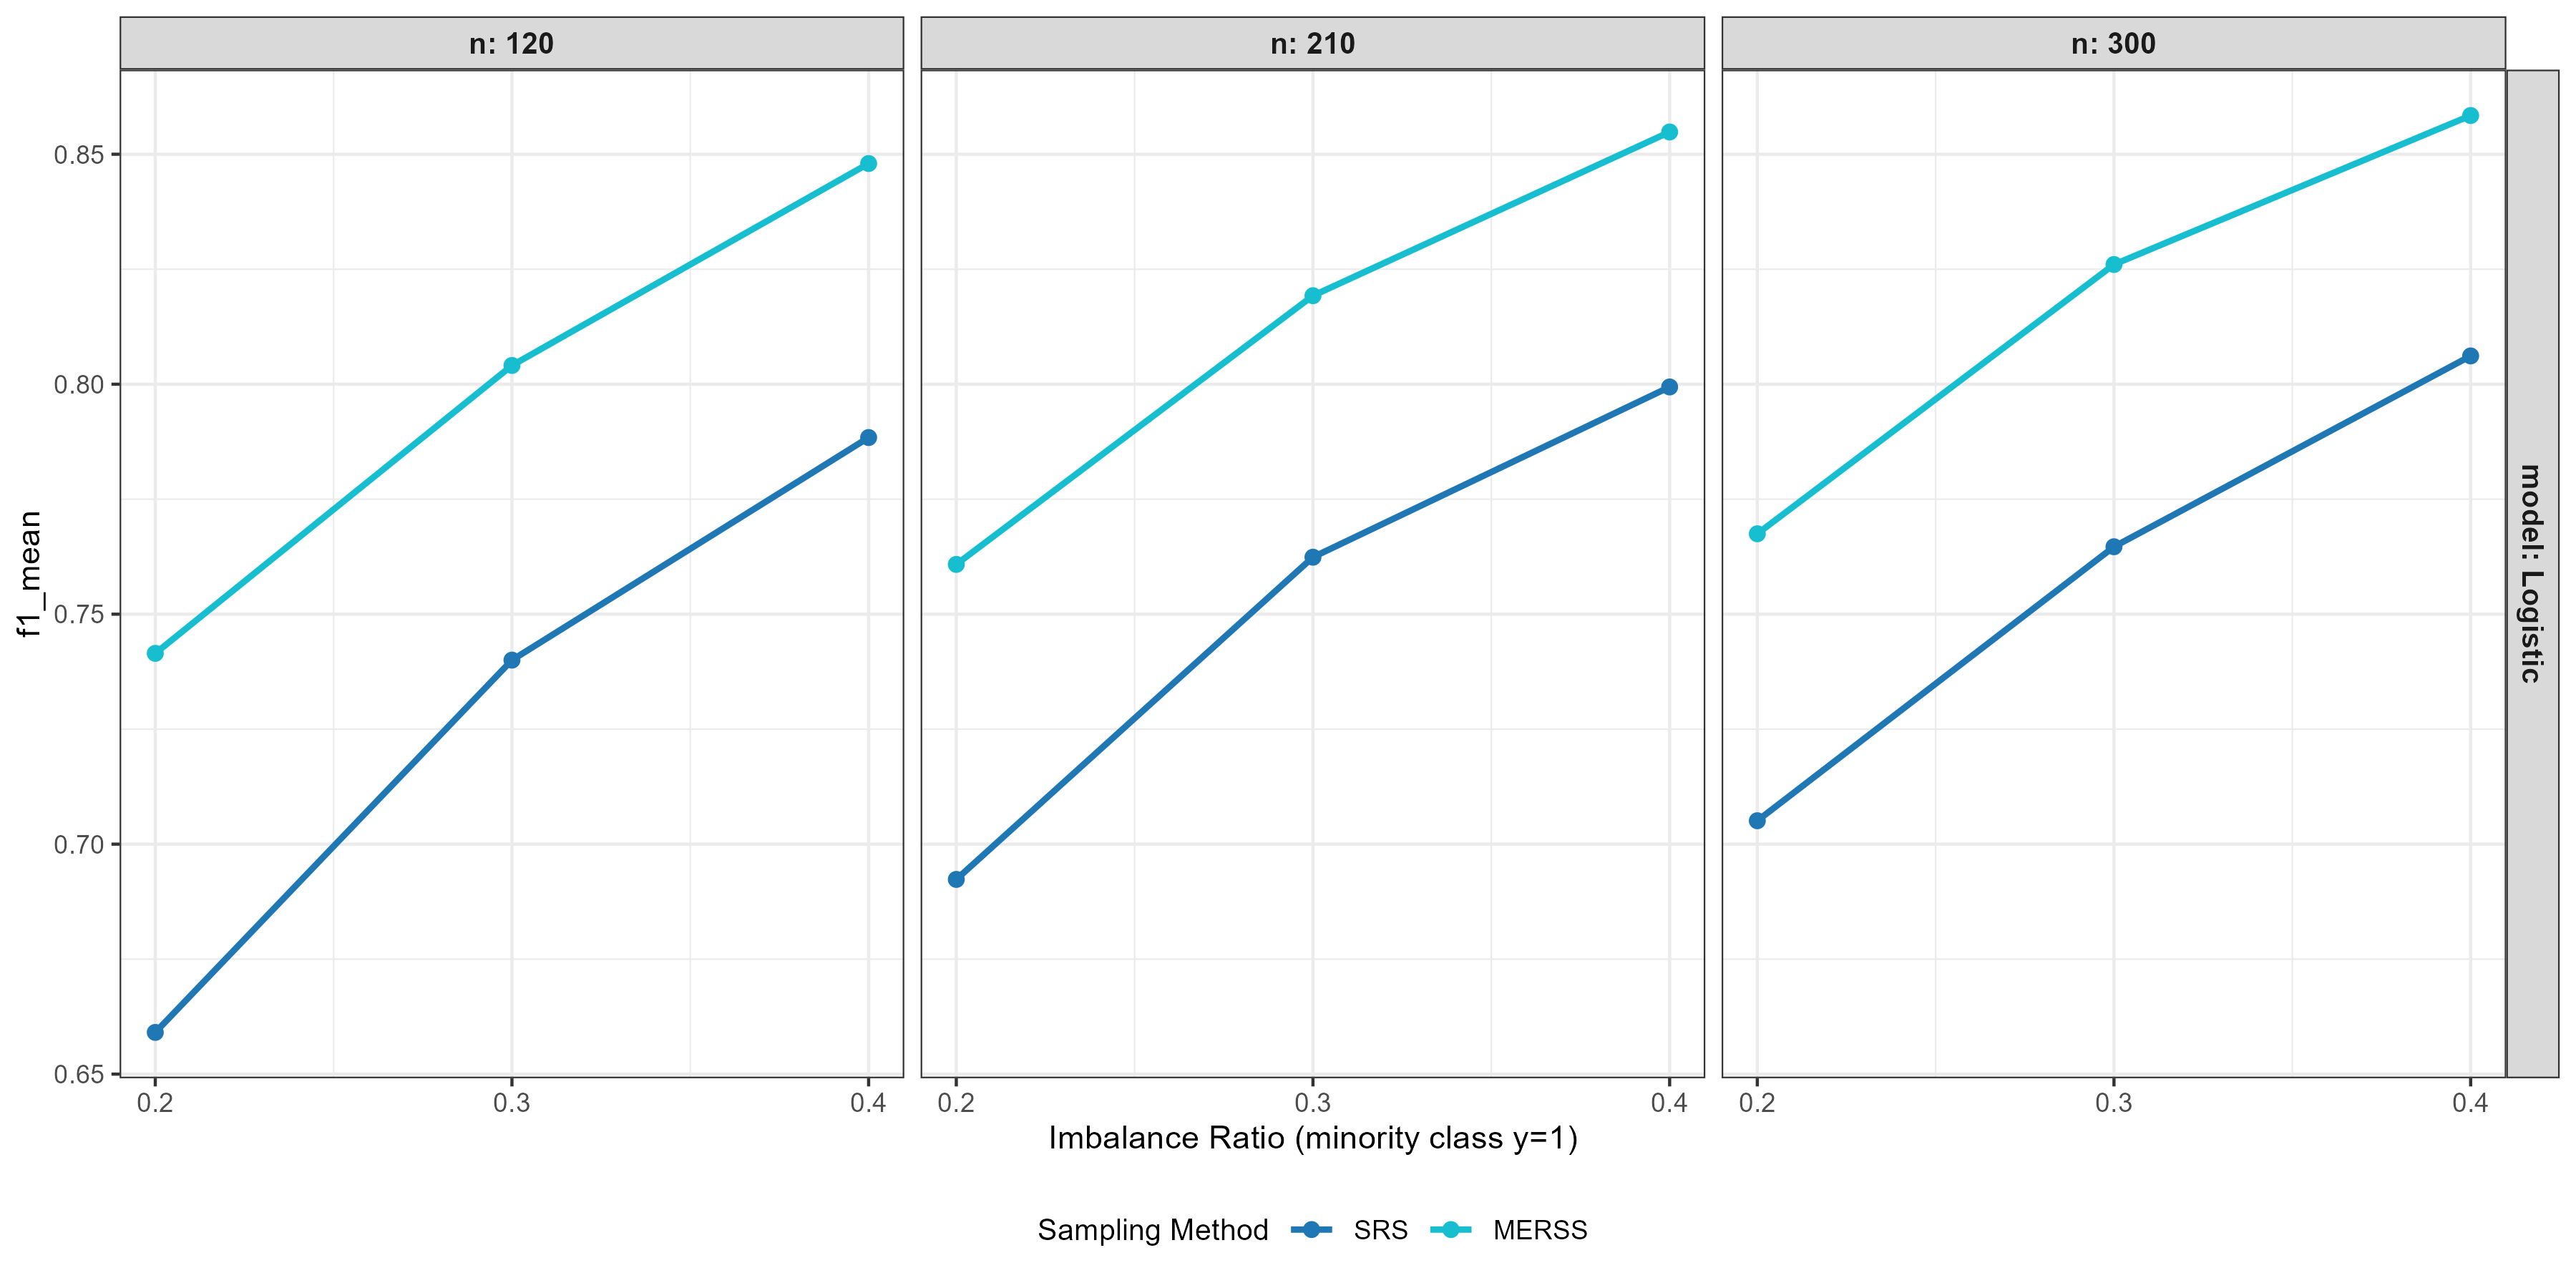
\includegraphics[width=0.40\textwidth]{Images/Coeff0.5_k3.png}\label{fig:f1_a}}
\hfill
\subfloat[\(k = 5\)]{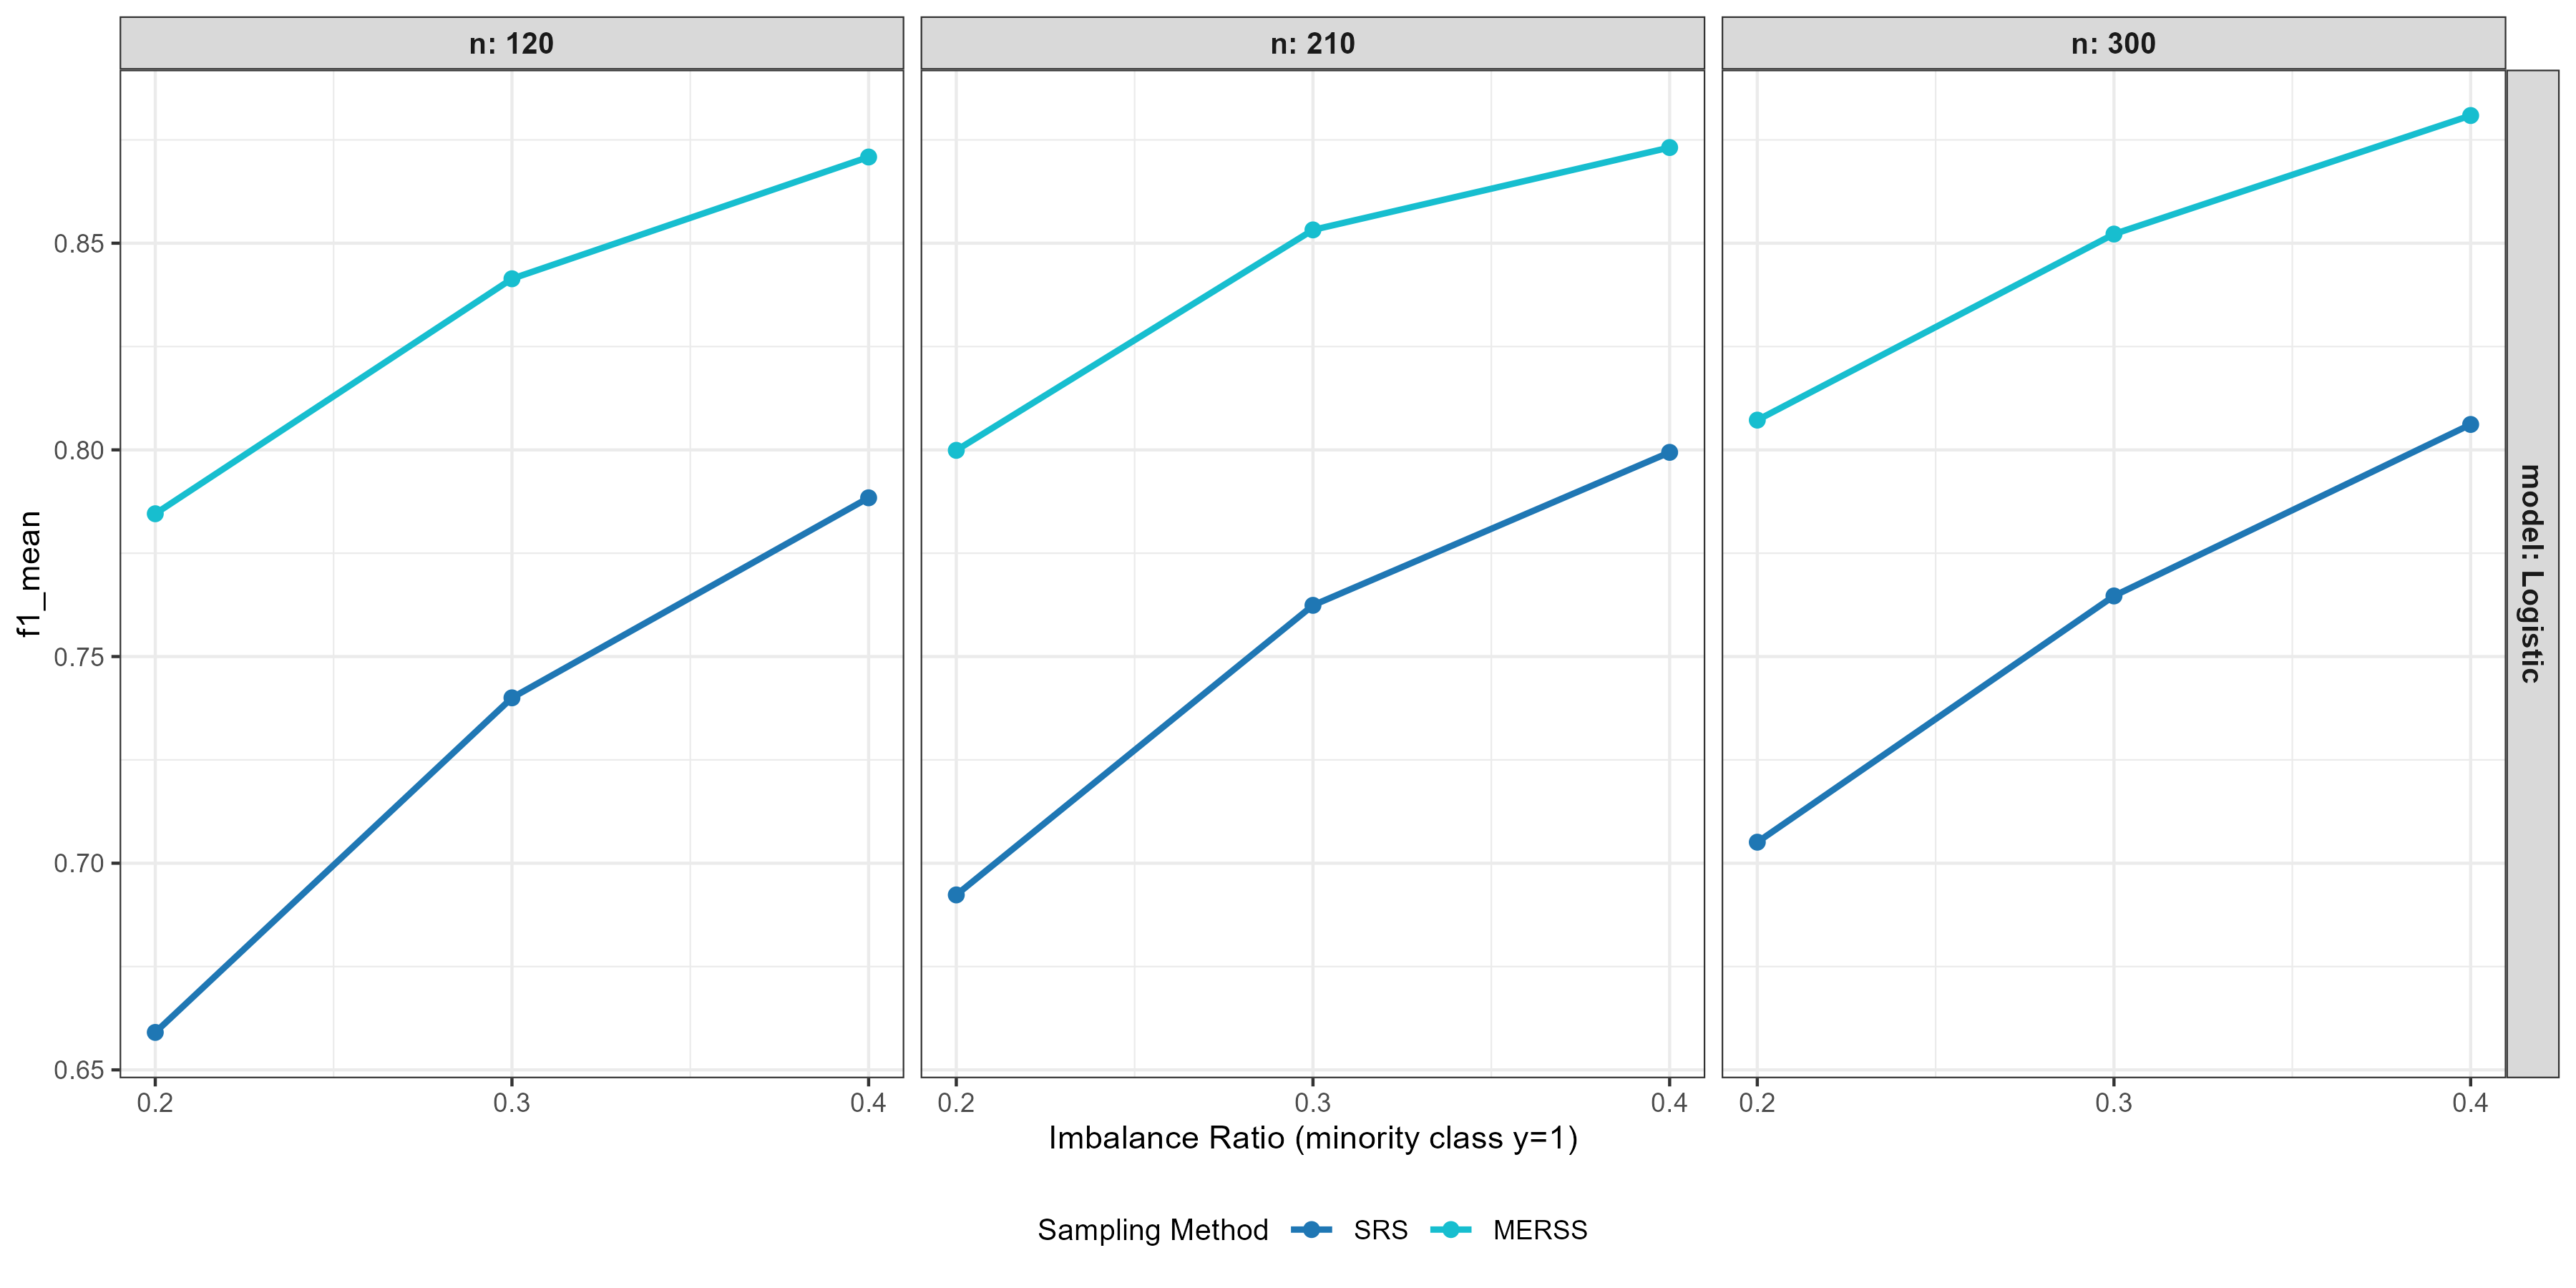
\includegraphics[width=0.40\textwidth]{Images/Coeff0.5_k5.png}\label{fig:f1_b}}
\hfill
\subfloat[\(k = 10\)]{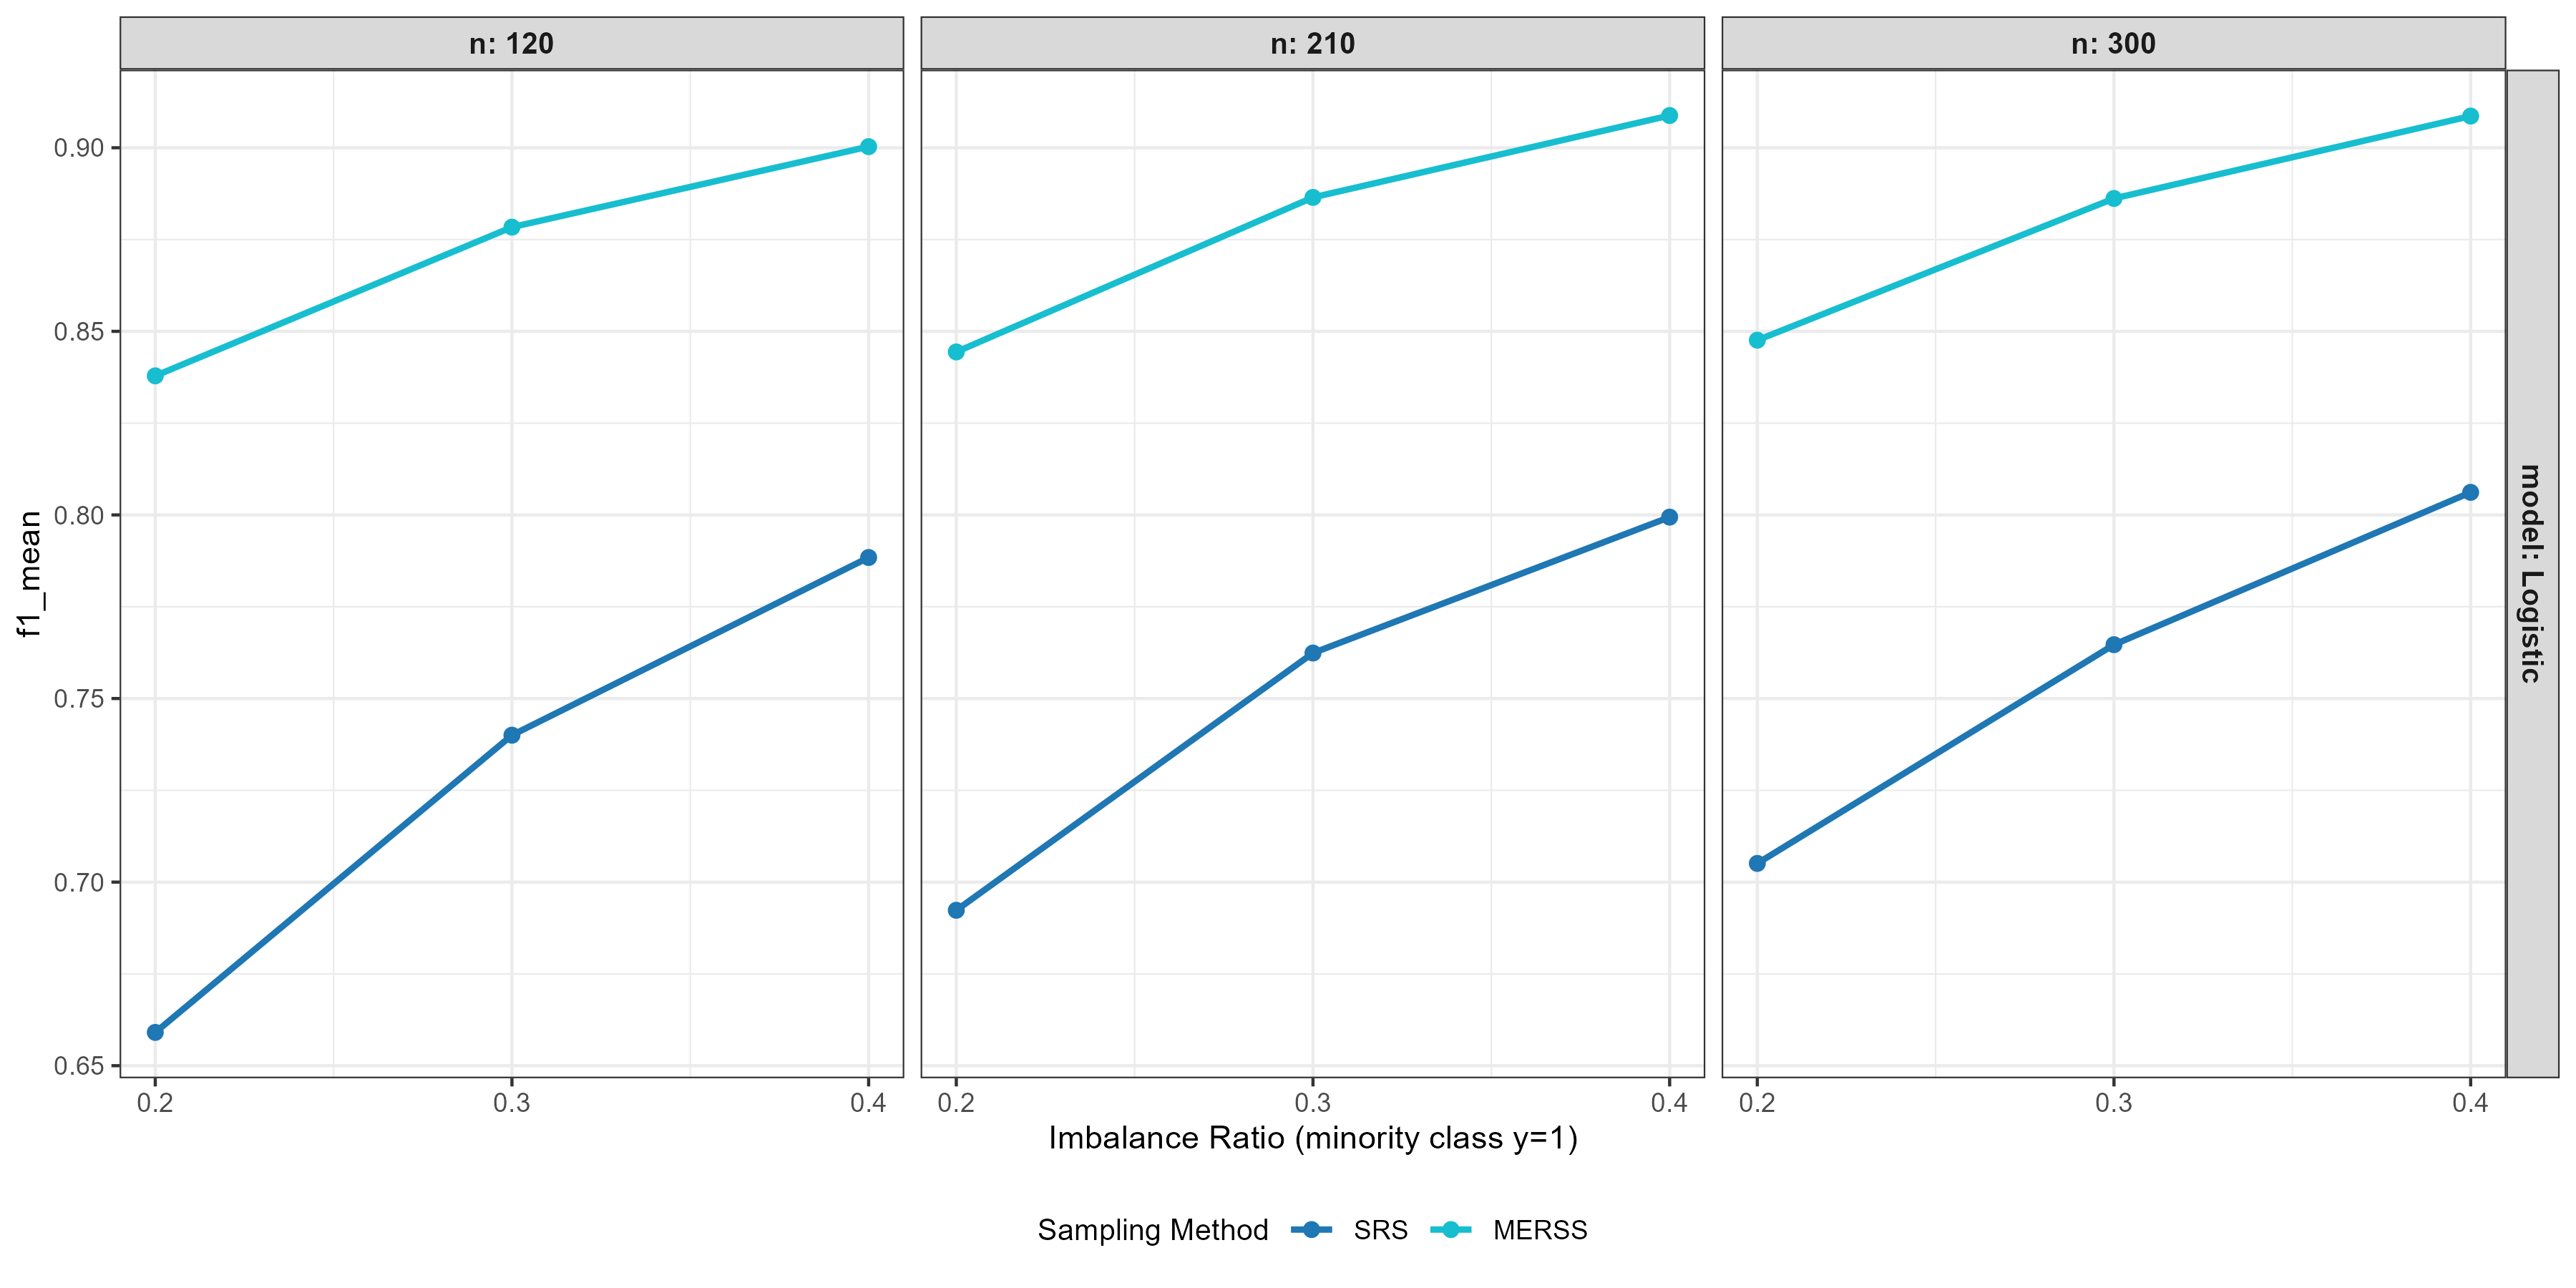
\includegraphics[width=0.40\textwidth]{Images/Coeff0.5_k10.png}\label{fig:f1_c}}
\caption{Minor-F1 score for MERSS vs. SRS at \(\rho = 0.5\) across different sample sizes and set sizes.}
\label{fig:f1_comparison}
\end{figure}
%%%%%%%%%%%%%%%%%%%%%%%%%%%%%%%%%%%%%%%%


\textbf{Effect of Correlation (\(\rho\)) and Sample Size (\(n\)).}
Higher \(\rho\) and larger \(n\) improved all metrics for both methods. MERSS consistently matched or exceeded SRS across all \(\rho\) levels (0.3, 0.5, 0.7) and all sample sizes (\(n = 120, 210, 300\)), with the clearest separation observed at moderate correlations (\(\rho = 0.5\)), as demonstrated in Figures~\ref{fig:f1_a}--\ref{fig:f1_c}.



%%%%%%%%%%%%%%%%%%%%%%%%%%%%%%%%%%%%%%%%%%%%%%%%%%%%%%%%%%%%%%%%%%%%%%%%%%%%%%%%%%%%%%%%%%%%%%%%%%%%%%%%

%%%%%%%%%%%%%%%%%%%%%%%%%%%%%%%%%%%%%%%%%%%%%%%%%%%%%%%%%%%%%%%%%%%%%%%%%%%%%%%%%%%%%%%%%%%%%%%%%%%%%%%%

\section*{Discussion and Conclusion}   

This study evaluated the performance of MERSS for LR classification under imbalanced conditions. Our results demonstrated that MERSS consistently outperforms SRS, particularly for minority class identification. These findings align with previous research demonstrating the efficiency of RBS methods \cite{Santos2017, Yousefi2026} and extend the work of Samawi et al. \cite{Samawi2017, Samawi2020} by focusing specifically on classification performance rather than parameter estimation.

The advantages of MERSS were most pronounced under severe imbalance (\(r = 0.2\)) and moderate to high correlation (\(\rho = 0.5, 0.7\)), where improvements in Precision and Minor-F1 reached up to 15\% and 29\%, respectively, compared to SRS. Increasing set size (\(k\)) from 3 to 10 consistently enhanced MERSS performance, consistent with Samawi et al. \cite{Samawi2017}, \cite{Santos2017}, and \cite{Yousefi2026}. Notably, these gains were achieved with no additional computational cost, supporting the practical utility of MERSS in resource-limited settings.

On the other hand, unlike synthetic data methods such as SMOTE \cite{Elreedy2024}, MERSS selects actual observational units using auxiliary information, preserving data authenticity while enriching minority class representation. This characteristic makes MERSS particularly valuable in different research where data integrity and inferential validity are paramount.

In conclusion, MERSS reliably enhances LR classification under imbalance, improving minority class identification at no additional computational cost. The method is most effective with moderate to strong auxiliary correlation and larger set sizes. These findings establish MERSS as a practical sampling strategy for rare event research with limited resources.
%%%%%%%%%%%%%%%%%%%%%%%% References %%%%%%%%%%%%%%%%%%%%%%%%%%%%%

\begin{thebibliography}{9}

\bibitem[Hosmer et al.(2013)]{Hosmer2013} Hosmer Jr DW, Lemeshow S, Sturdivant RX. Applied logistic regression: John Wiley \& Sons; 2013.

\bibitem[Noor et al.(2022)]{Noor2022} Noor S, Tajik O, Golzar J. Simple random sampling. International Journal of Education \& Language Studies. 2022;1(2):78-82.

\bibitem[McIntyre (1952)]{McIntyre1952} McIntyre G. A method for unbiased selective sampling, using ranked sets. Australian journal of agricultural research. 1952;3(4):385-90.

\bibitem[Al-Odat and Al-Saleh(2001)]{AlOdat2001} Al-Odat M, Al-Saleh MF. A variation of ranked set sampling. Journal of Applied Statistical Science. 2001;10:137-46.

\bibitem[Samawi et al.(2017)]{Samawi2017} Samawi HM, Rochani H, Linder D, Chatterjee A. More efficient logistic analysis using moving extreme ranked set sampling. Journal of Applied Statistics. 2017;44(4):753-66.

\bibitem[Samawi et al.(2020)]{Samawi2020} Samawi HM, Zhang X, Rochani H. Further Improving the Performance of Logistic Regression Analysis Using Double Extreme Ranking. Journal of Statistical Theory and Practice. 2020;14:1-16.

\bibitem[Santos and Barrios (2017)]{Santos2017} Santos KCP, Barrios EB. Improving predictive accuracy of logistic regression model using ranked set samples. Communications in Statistics-Simulation and Computation. 2017;46(1):78-90.

\bibitem[Yousefi et al.(2026)]{Yousefi2026} Yousefi R, Liquet B, Mahdizadeh M, Tapak L, Doosti H, Esmaily H. Enhancing logistic regression classification: insights from simulation and real-world applications through ranked set sampling. Scientific Reports. 2026;16(1):11938.

\bibitem[Elreedy et al.(2024)]{Elreedy2024} Elreedy D, Atiya AF, Kamalov F. A theoretical distribution analysis of synthetic minority oversampling technique (SMOTE) for imbalanced learning. Machine Learning. 2024;113(7):4903-23.
\end{thebibliography}
 \end{document}

